% Modelo de relatório no estilo artigo em duas colunas
\documentclass[twocolumn]{article}
\usepackage[utf8]{inputenc}
\usepackage{amsmath}
\usepackage{subcaption}
\usepackage{mathtools}
\usepackage{graphicx}
\usepackage{color}
\usepackage{authblk}
\usepackage{lmodern}
% \usepackage[colorlinks,citecolor=black,urlcolor=black,bookmarks=false,hypertexnames=true]{hyperref}
\usepackage{geometry}
\usepackage{pdfpages}
\usepackage{fancyhdr}
\usepackage[utf8]{inputenc}

\usepackage[sorting=none,style=numeric]{biblatex}
\addbibresource{refs.bib}
\usepackage[justification=centering]{caption}
\usepackage{makecell}
\usepackage{booktabs}
\usepackage{hhline}
\usepackage{amsmath}
\usepackage{amssymb}
\usepackage{soul}
\usepackage{gensymb}
\usepackage{listings}

\setlength\parindent{0pt}


\newcommand{\myname}{Nishant Aswani}
\newcommand{\mynetid}{nsa325}
\newcommand{\myemail}{nsa325@nyu.edu}
\newcommand{\myhwtype}{Lab }
\newcommand{\myhwnum}{3}
\newcommand{\mycoursenumber}{ENGR-UH 3511}
\newcommand{\myclassname}{Computer Organization and Architecture}
\newcommand{\myassignmenttitle}{Microprocessor Design and Verilog HDL: Part 1}
\newcommand{\myinstructor}{Cristoforos Vasilatos}

\newcommand{\cc}[1]{\texttt{#1}}

\lstset{
  basicstyle=\ttfamily,
  escapeinside=||
}

% Tamanho das margens:
% \geometry{
% 	a4paper,
% 	total={170mm,257mm},
% 	left=30mm,
% 	top=20mm,
% }
%%%%%%%%%%%%%%%%%%%%%%%%%%%%%%%%%%%%%%%%%
% Bibliografia estilo ABNT. Se não tiver instalado, comente a linha abaixo.
% \usepackage[alf, abnt-etal-list=0, abnt-emphasize=bf,abnt-last-names=bibtex, abnt-etal-text=it, abnt-etal-cite=2]{abntex2cite}
%%%%%%%%%%%%%%%%%%%%%%%%%%%%%%%%%%%%%%%%%

% Dados de identificação
\title{\myassignmenttitle}
\author{\myname, \myemail}
\affil{\myclassname (\mycoursenumber), Instructor \myinstructor}
\date{}

\begin{document}
%%%%%%%%%%%%%%%%%%%%%%%%%%%%%%%%%%%%%%%%%%%%%%%% COVER PAGE %%%%%%%%%%%%%%%%%%%%%%%%%%%%%%%%%%%%%%%%%%%%%%%%%%%%
\onecolumn
\pagestyle{fancy}
\fancyhf{}
\renewcommand{\headrulewidth}{0pt}
\rhead{\textbf{Division of Engineering}}
\lhead{\textbf{NYU Abu Dhabi}}

\begin{center}
  
\includegraphics[scale=0.15]{etc/NYUAD-alt-logo.jpg}
\end{center}

{\vspace{2.5em}}

\begin{center}
    \Huge{\textbf{\mycoursenumber}}\\
    {\vspace{0.5em}}
    \Huge{\textbf{\myclassname}}
\end{center}

{\vspace{10em}}

\begin{center}
  \begin{tabular}{|rp{5.0cm}lll|}
    \hline
    &  &  &  & \\
    &  &  &  & \\
    \Large{\textbf{Name:}} & \Large{\myname}
    
    \  &  &  & \\
    \Large{\textbf{Net ID:}} & \Large{\mynetid}
    
    \  &  &  & \\
    \Large{\textbf{Assignment Title:}} & \Large{\myhwtype \myhwnum}
    
    \
    
    \  &  &  & \\
    \hline
  \end{tabular}
\end{center}

\

{\newpage}
%%%%%%%%%%%%%%%%%%%%%%%%%%%%%%%%%%%%%%%%%%%%%%%% COVER PAGE %%%%%%%%%%%%%%%%%%%%%%%%%%%%%%%%%%%%%%%%%%%%%%%%%%%%

\maketitle        

% Resumo de no máximo 200 palavras
% \begin{abstract}
% Este documento orienta a descrição das atividades práticas desenvolvidas em laboratório. São usados como exemplo conceitos da Aula 01 de Acionamentos Elétricos sobre partida direta de motor de indução trifásico. Nesta atividade, um motor é acionado com conexões estrela e triângulo a vazio. As correntes nominais e de partida são medidas com amperímetro analógico e comparadas entre si. Nota-se que, mesmo sem carga, as corrente em estrela são maiores. 
% \end{abstract}

\section{Introduction}

The MIPS architecture falls under the reduced instruction set computer (RISC) family of instruction set architectures (ISAs). MIPS is a 32-bit architecture, employing 32 registers, each 32 bits wide. Verilog is a hardware description language, used to model hardware systems. Unlike C/C++, Verilog operates on modules and processes, the latter of which run in parallel, instead sequentially. \\  

The following lab uses Verilog to begin an implementation of a 32-bit MIPS CPU. The modules implemented include a program counter, instruction memory, register file, ALU, and data memory. 

\section{Methodology}

Icarus Verilog was used as a compiler to produce the object files for all verilog modules. The object file was then simulated using the \cc{vvp} command from Icarus Verilog. The final output was viewed in GTKwave. \\

A make file was written to compile all .v files in the testbench folder. The makefile then runs \cc{vvp} and \cc{gtkwave}. 

\newpage

\section{Results}

\subsection{Program Counter}

Below is the implementation of the program counter, with the test bench on the left. As seen in the \cc{always@} block, the logic simply adds 4 to the value of the input address to give the next instruction address. Hence, there is a clock input, an input address, and an output address.  

\begingroup
    \centering
    \medskip
    %width=\columnwidth
    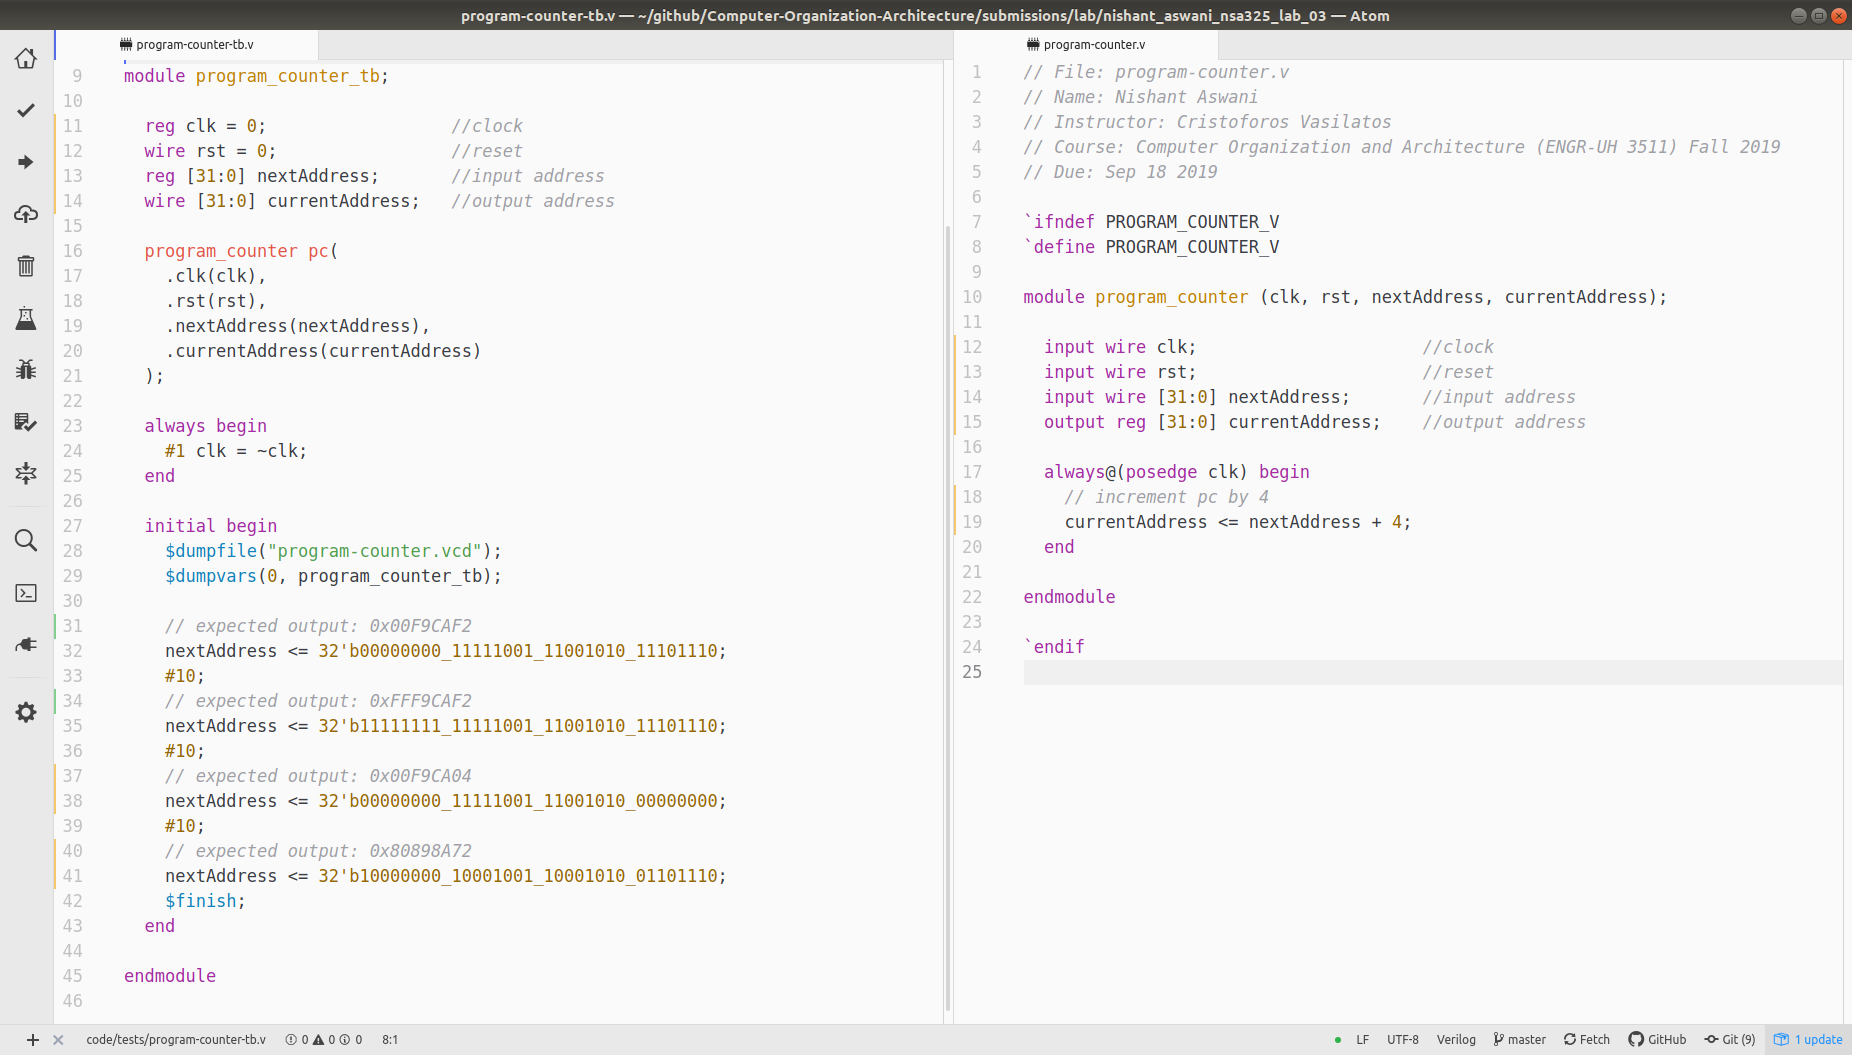
\includegraphics[width=\columnwidth]{Lab-Tex/Lab3-images/program-counter.png}
    \captionof{figure}{Verilog implementation of program counter with its testbench}
    \medskip
\endgroup

The test bench simply defines a clock that alternates every unit of time. Next, it sends four different address, each time expecting an output that is 4 greater than the input.\\

The variable nextAddress refers to the input address, while the variable currentAddress refers to the output. As seen below, an input value, 0x00F9CAEE, is fed using "nextAddress". Adding four to the input value results in 0x00F9CAF2, which is displayed by the "currentAddress" module. Similarly, the program counter outputs input+4 at the positive edge of the upcoming clock cycle for each of the inputs. \\


\begingroup
    \centering
    \medskip
    %width=\columnwidth
    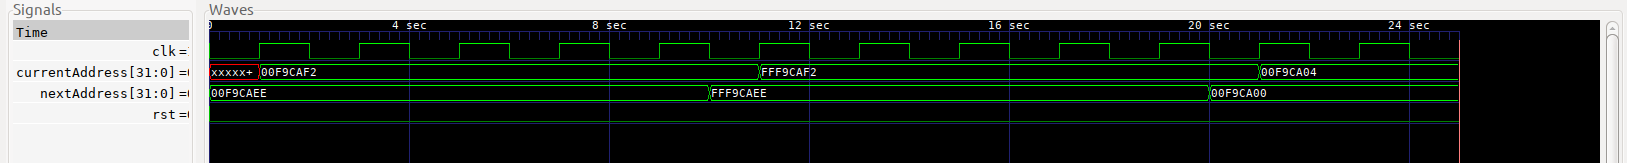
\includegraphics[width=\columnwidth]{Lab-Tex/Lab3-images/program-counter-wave.png}
    \captionof{figure}{Waveform for program counter}
    \medskip
\endgroup

\subsection{Instruction Memory}

To simulate memory, we use an array of 32 bit registers and instantiate a few of them with dummy instructions for demonstration purposes. Otherwise, the module simply takes in an address value, which is fed into the array as an index. It then retrieves the stored instruction. \\

The testbench asks for the instructions in registers 1, 2, 3, and 0 respectively. For example, registers 2 and 3 store hex values \cc{0x8BADFOOD} and \cc{0xDEADBABE}, which can be seen in the middle in the \cc{gtkwave} screenshow below. Since the instruction memory is not driven by the positive edge of the clock in this implementation, it is able to retrieve the instruction without a clock cycle delay. \\

\begingroup
    \centering
    \medskip
    %width=\columnwidth
    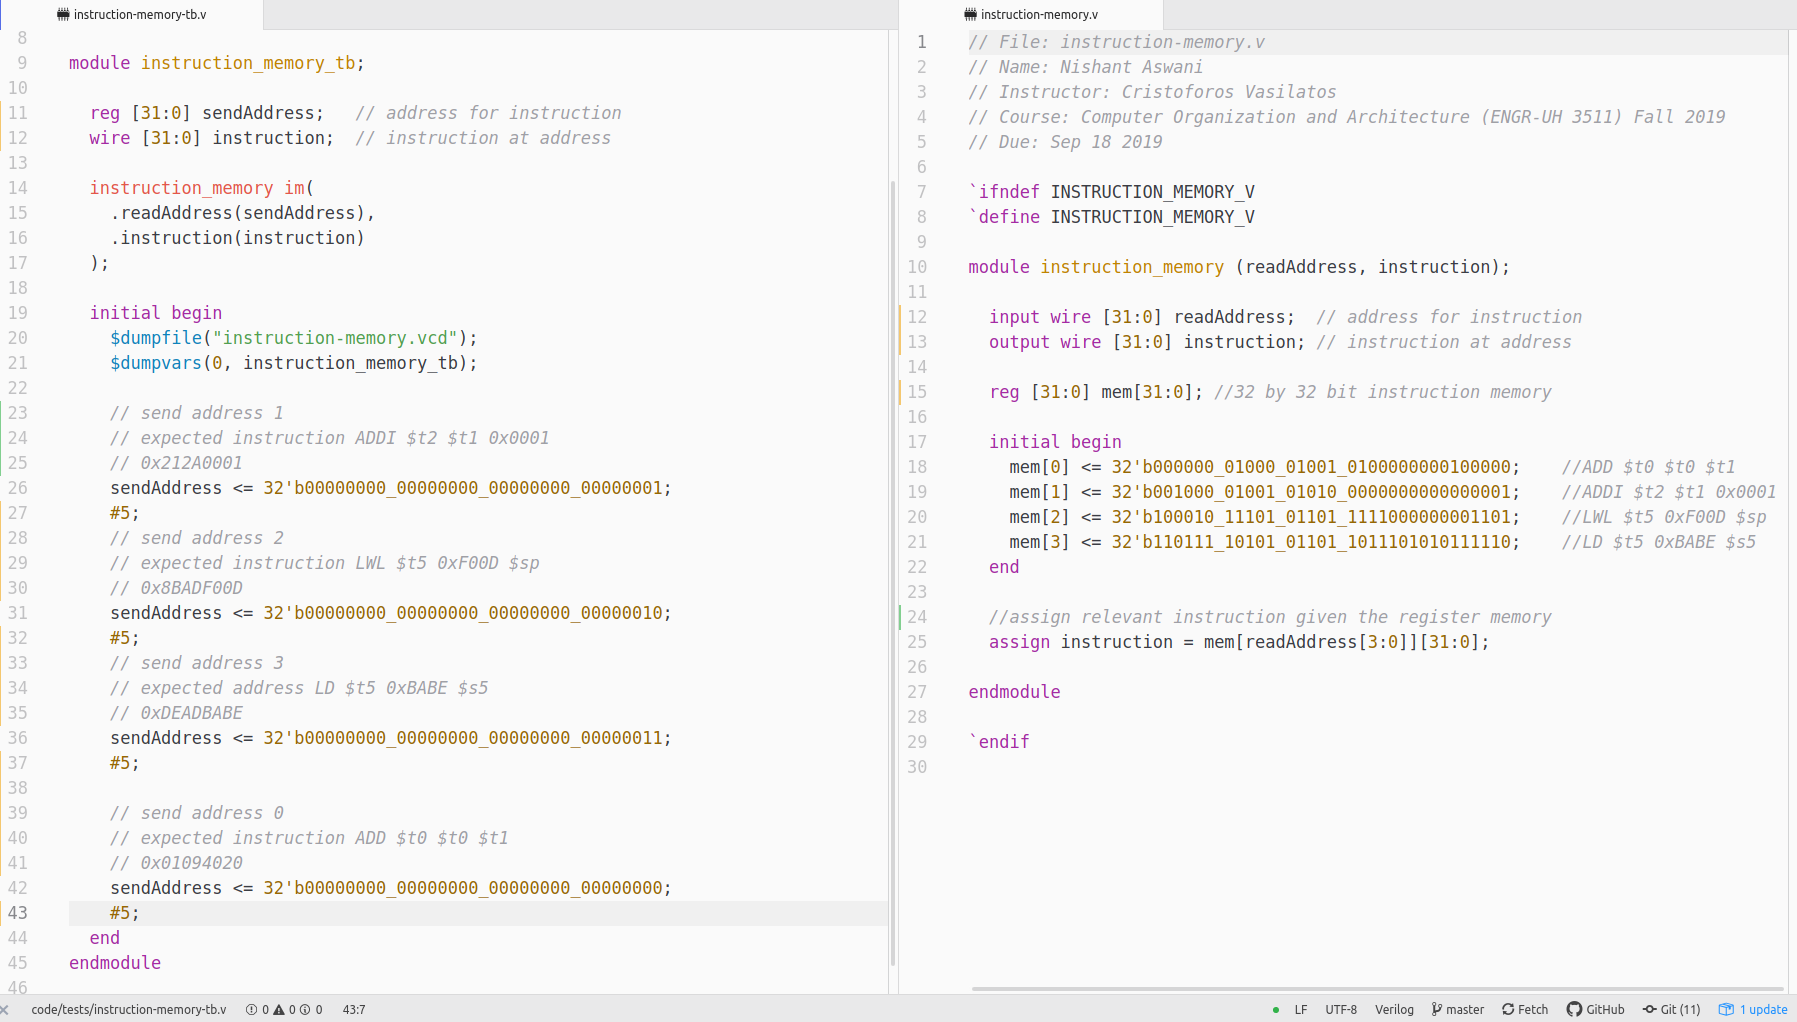
\includegraphics[width=\columnwidth]{Lab-Tex/Lab3-images/instruction-memory.png}
    \captionof{figure}{Verilog implementation of instruction memory with its testbench}
    \medskip
\endgroup
\medskip

\begingroup
    \centering
    \medskip
    %width=\columnwidth
    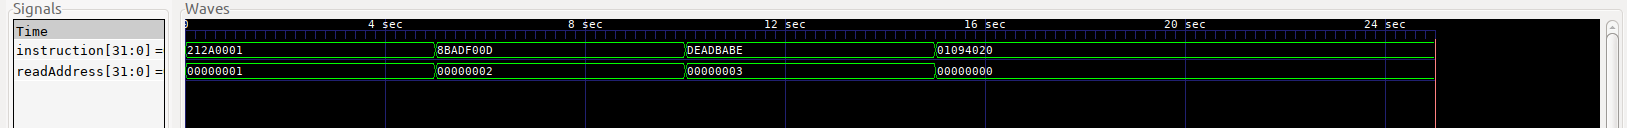
\includegraphics[width=\columnwidth]{Lab-Tex/Lab3-images/instruction-memory-waveform.png}
    \captionof{figure}{Waveform for instruction memory}
    \medskip
\endgroup

\newpage

\subsection{Register File}

The register file is the part of the CPU which stores 32 registers, each 32 bits wide. The module accepts 5 bit addresses for three registers (two for reading and one for writing). It also accepts 32 bits for the data to be written into the specified register. Moreover, there is a write enable control signal. Finally, the register file has two outputs, each 32 bits, which carry the value stored in the read addresses provided. Traditionally, these 32 bit values are sent off to the ALU for processing.\\ 

The module instantiates a 2D array for registers. Then, at each positive edge of the clock, it first checks for the reset signal. If reset is enabled, all registers are set to 0. Otherwise, it checks for the writeEnable to decide for or against storing the provided write data. At the end of this if/else block, the readData wires are assigned the corresponding values from the register file. \\

\begingroup
    \centering
    \medskip
    %width=\columnwidth
    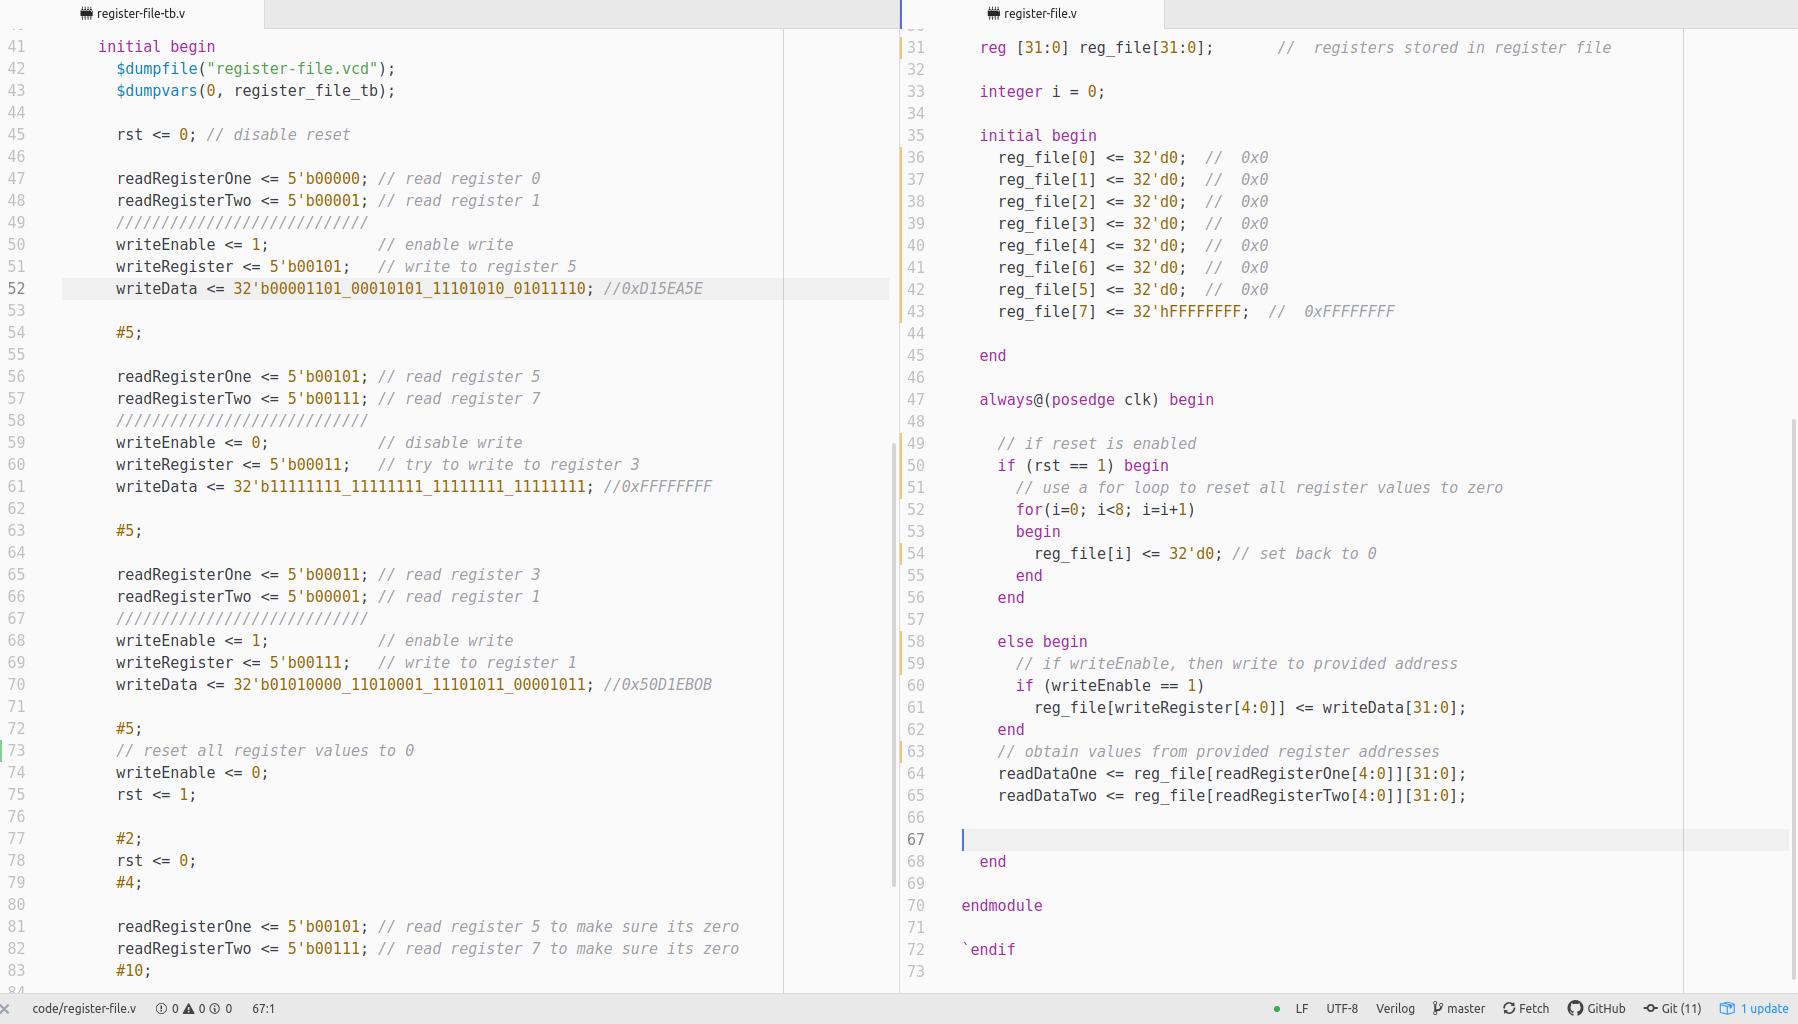
\includegraphics[width=\columnwidth]{Lab-Tex/Lab3-images/register-file.png}
    \captionof{figure}{Verilog implementation of register file with its testbench}
    \medskip
\endgroup
\medskip

Notice in the implementation that all registers are instantiated with value 0, except register 7 which holds \cff{0xFFFFFFFF}. This is for demonstration purposes. Looking at the output, in the first cycle, we write the value \cc{0xD15EA5E} to register 5. In the next cycle, we read register 5 and 7. Accordingly, the readDataOne and readDataTwo output \cc{0xD15EA5E} and \cff{0xFFFFFFFF}, respectively.  \\

\begingroup
    \centering
    \medskip
    %width=\columnwidth
    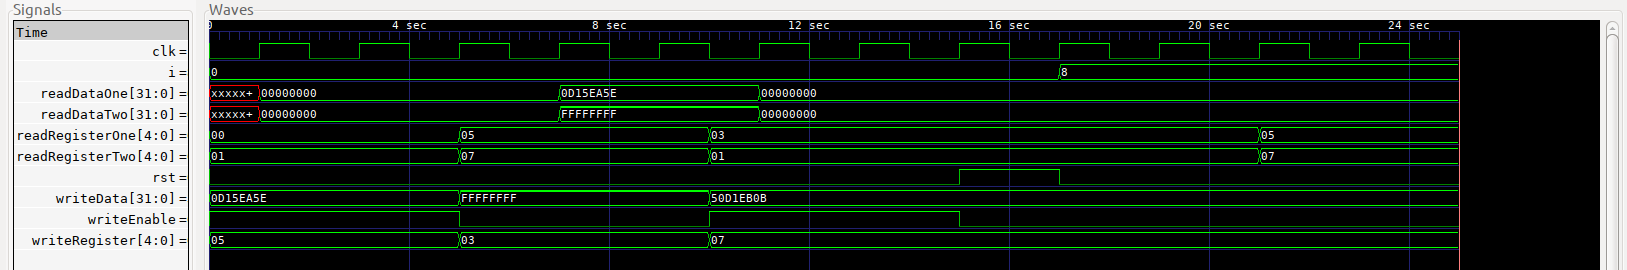
\includegraphics[width=\columnwidth]{Lab-Tex/Lab3-images/register-file-wave.png}
    \captionof{figure}{Waveform for the register file module}
    \medskip
\endgroup
\medskip

Within the same cycle, the code attempts to write to register 3. However, we see in the next cycle that register 3 remains unchanged, because the writeEnable signal was not turned on. Finally, the last cycle reflects the effects of enabling the reset buttons: register 5 and 7 have been reset to 0. 

\subsection{ALU}

The ALU is driven by a clock and carries out an operation, specified by the function code, on two 32-bit values. It then outputs the resulting 32-bit value along with a flag which conveys whether the result is 0 or not. \\

As a result, the ALU implementation is a simple switch case, carrying out the operation corresponding to the function code. Finally, it carries out a simple if/else check for the zero flag. \\

\begingroup
    \centering
    \medskip
    %width=\columnwidth
    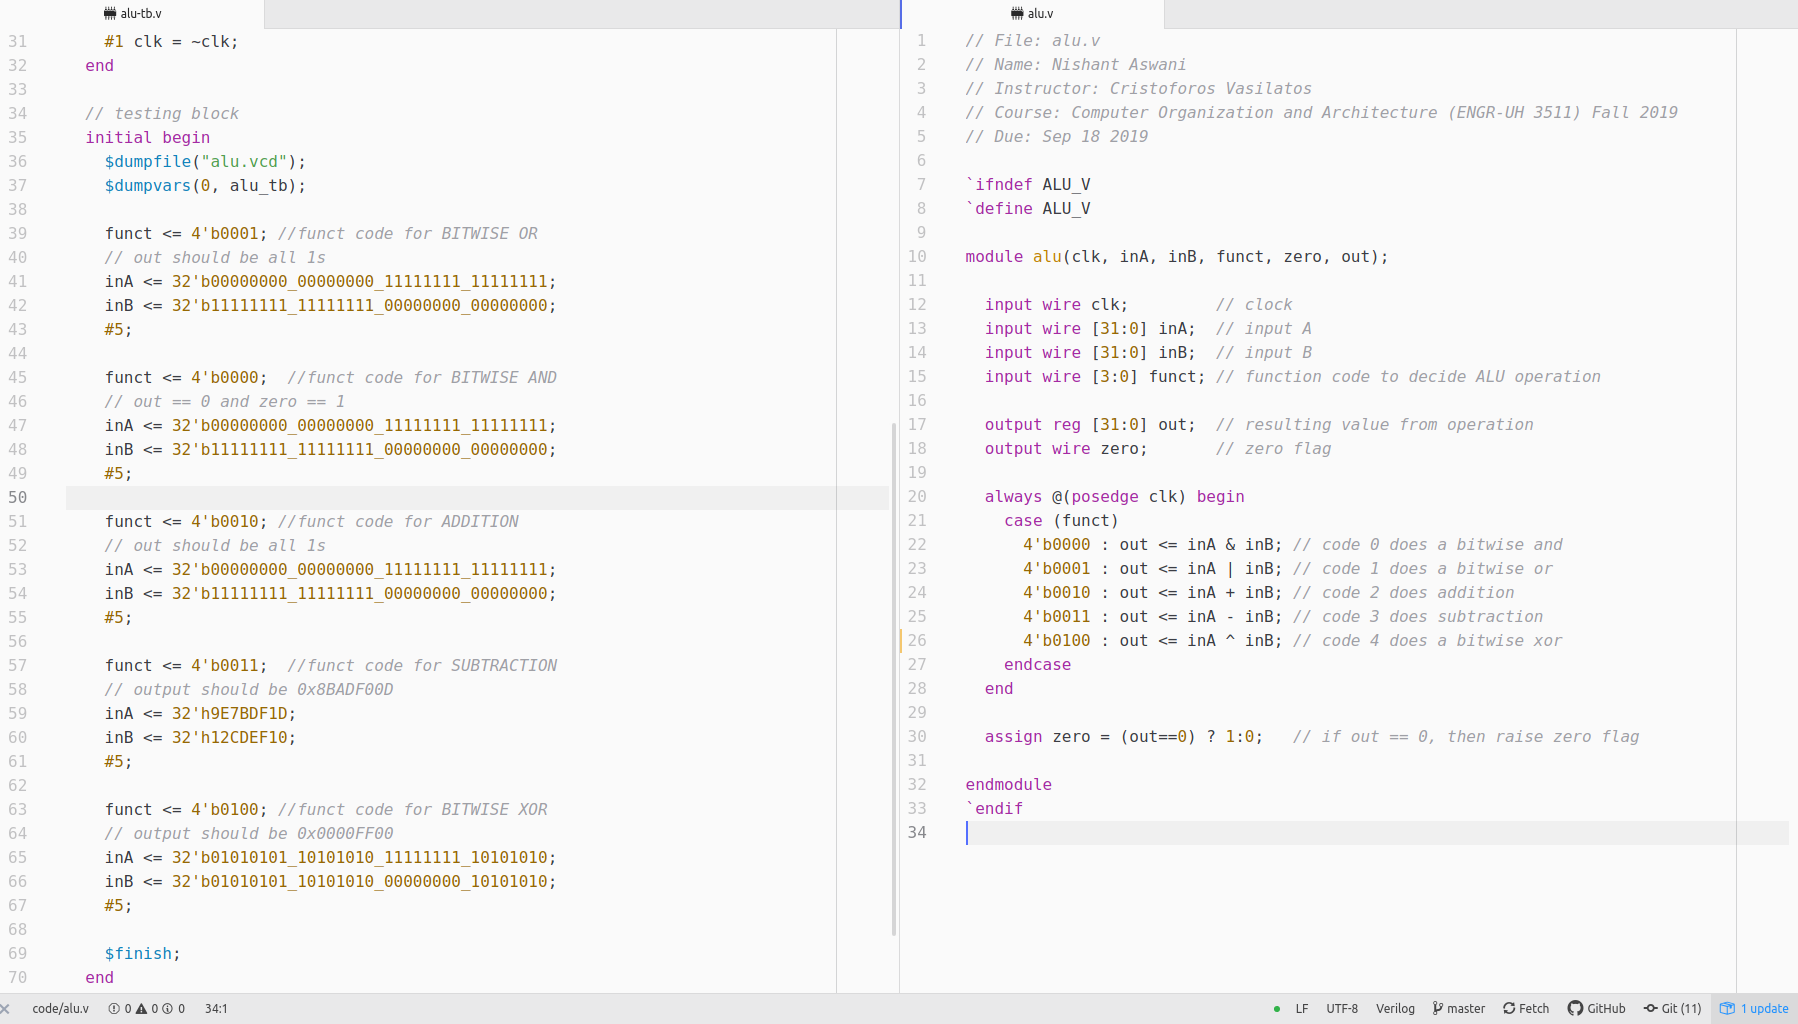
\includegraphics[width=\columnwidth]{Lab-Tex/Lab3-images/alu.png}
    \captionof{figure}{Verilog implementation of ALU with its testbench}
    \medskip
\endgroup
\medskip
\\

In the test bench, we carry out the bitwise AND and the bitwise OR operations with A = 0x0000FFFF and B = 0xFFFF0000. As expected, the output wave shows 0xFFFFFFFF and 0x00000000 for the respective operations. Notice, the zero flag is enabled for the second result. The remaining inputs demonstrate the functionality for the remaining operations (addition, subtraction, and bitwise XOR).\\

\begingroup
    \centering
    \medskip
    %width=\columnwidth
    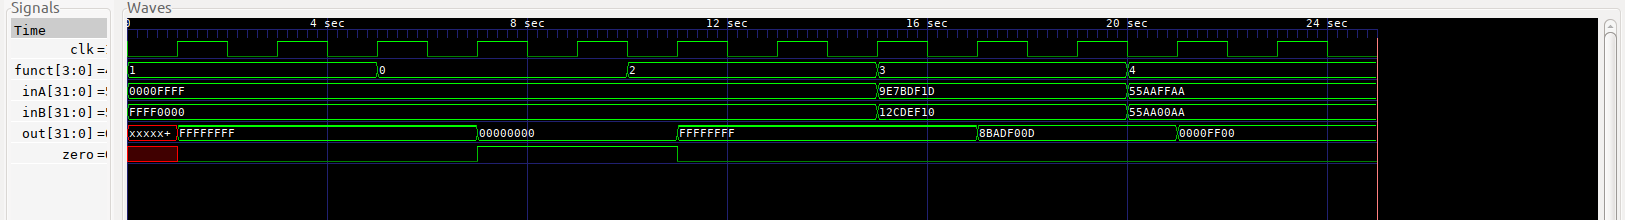
\includegraphics[width=\columnwidth]{Lab-Tex/Lab3-images/alu-wave.png}
    \captionof{figure}{Waveform of the ALU module}
    \medskip
\endgroup
\medskip

\subsection{Data Memory}
\\
Driven by a clock, the data memory receives an address to which it either reads or writes. Hence, there are two control signals memRead and memWrite, which decide the operation of the data memory. Given that memWrite is enabled, the data memory also accepts a 32-bit value to write to the given address.  \\

This data memory implementation simulates memory by using registers, which are instantiated with some random values. At the positive edge of each clock cycle, if memWrite is enabled, the module writes to the given address. It then checks for the memRead signal and outputs 0 if it is disabled. \\

\begingroup
    \centering
    \medskip
    %width=\columnwidth
    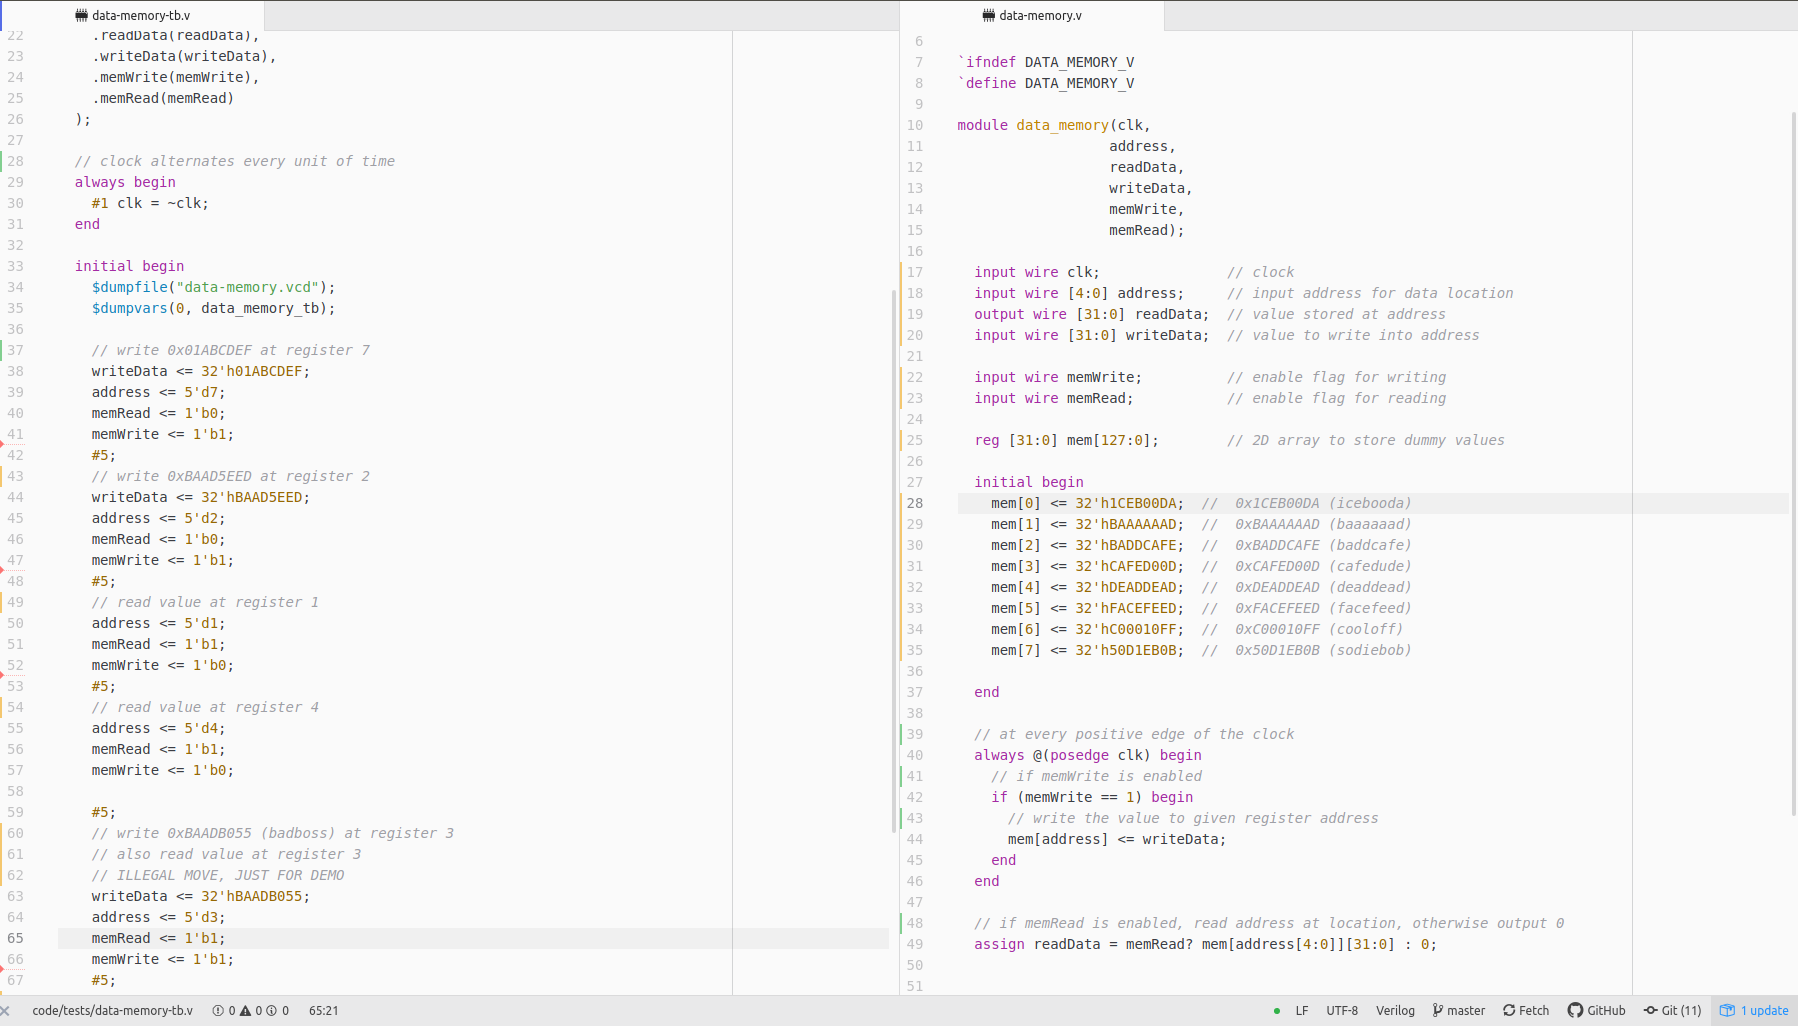
\includegraphics[width=\columnwidth]{Lab-Tex/Lab3-images/data-memory.png}
    \captionof{figure}{Verilog implementation of data memory with its testbench}
    \medskip
\endgroup
\medskip

\\

Looking at the testbench, we first write a value to the 7th registe. We then write another value to the 2nd register; both times the memWrite signal is enabled, so the write is successful. Notice that the readData signal outputs 0 because the memRead control is disabled. In the next two assignments, we read from registers 1 and 4. \\ 

\begingroup
    \centering
    \medskip
    %width=\columnwidth
    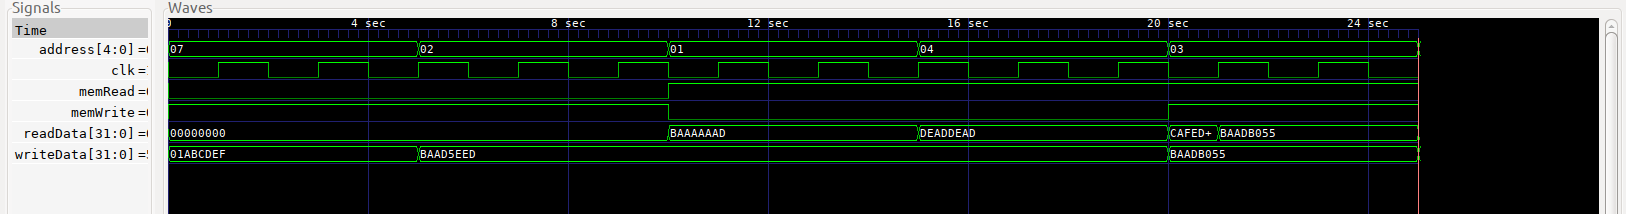
\includegraphics[width=\columnwidth]{Lab-Tex/Lab3-images/data-memory-wave.png}
    \captionof{figure}{Waveform of the data memory module}
    \medskip
\endgroup
\medskip

Finally, we attempt to read and write in the same cycle, which is an illegal move. The output waves demonstrates this issue, because the readData changes, giving two values within the same instruction cycle. This could adversely affect the CPU operation; hence, only one of the two control signals can be enabled at a given time. 

\section{Conclusion}

The above implementations generate the basic modules of the MIPS CPU. Future work involves connecting these modules as well as covering corner cases to allow robust functionality.



%%%%%%%%%%%%%%%%%%%%%%%%%%5
% BIBLIOGRAFIA 
% Estilo de bibliografia ABNT. Se não tiver instalado, mude para plain ou ieeetr

%\bibliographystyle{plain} % Inclua isso se não tiver ABNTEX instalado
% \begin{thebibliography}{refs}
% \bibitem{}
\printbibliography
% \end{thebibliography}
\end{document}